\chapter{Bilingual and multi-lingual baselines}

In this chapter we describe the baseline experiments.
Bilingual baselines are needed to specify the starting point:
how good can model perform on specific translation direction
for each test set.

After bilingual results are collected and inspected, it is time for
multi-lingual baselines. As multi-lingual baselines we consider models
with randomly selected set of target languages. This way we can see
how much adding more target languages to the model changes its performance
on the same specific translation direction.

Most of experiments are done on \gls{en-to-36} dataset with couple of
additional experiments on \gls{en-to-5}.




\section{\todo{Bilingual baseline}}
\label{section:bilingual_baseline}


We trained bilingual models on \gls{en-to-36} dataset and received
number of values for each translation direction.
Test results for relevant target directions (i.e. languages from
'Germanic' and 'Slavic with cyrillic script'
from Section \ref{subsection:proposed_experiments})
are shown in Table \ref{table:bilingual-results}.

\begin{figure}[h]
	\centering
	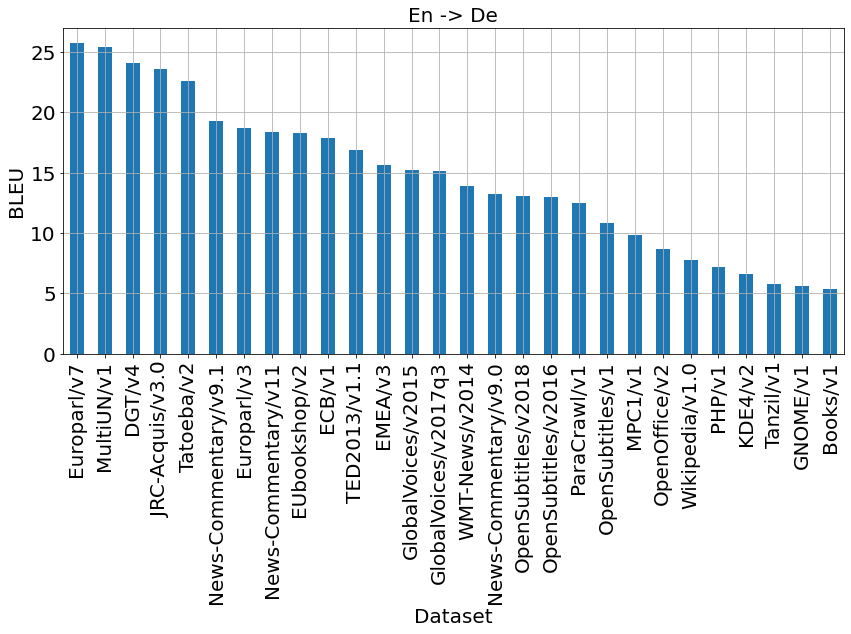
\includegraphics[width=0.9\columnwidth]{../img/bilingual_en_de.png}
	\mycaption{\dir{En}{De} bilingual results}{
		Datasets on the \emph{X} axis are sorted by declining BLEU score.
	}
	\label{fig:bilingual_en_de}
\end{figure}


\section{\todo{Multilingual baseline}}
\label{section:multilingual_baseline}

\begin{figure}[h]
	\centering
	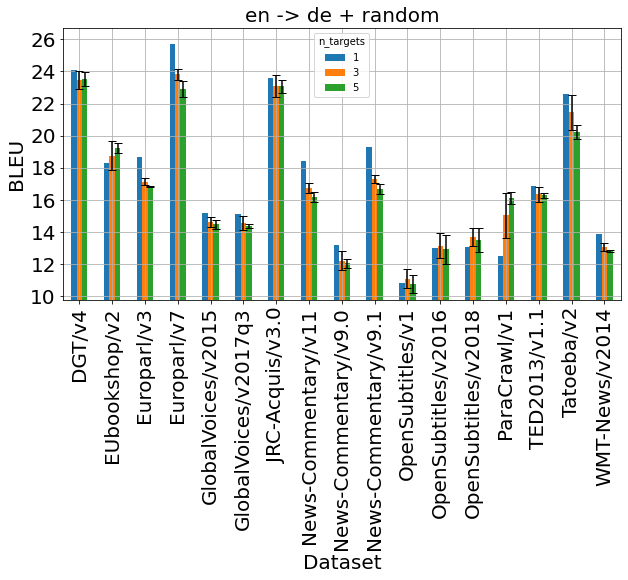
\includegraphics[width=1.0\columnwidth]{../img/random_en_de.png}
	\mycaption{En\to{}De monolingual baseline results (RANDOM)}{
		Datasets with BLEU lower than 10 are removed
	}
	\label{fig:random_en_de}
\end{figure}

E.g. as a bilingual baseline model for German target language the En\to{}De
model is trained.
En\to{}De,Fr, En\to{}${De,Az}$, En\to{}${De,Bg}$ En\to{}${Bg,Az}$ models
provide us with 3 results for En\to{}De direction 2-target baseline, as well
as one value for En\to{}Fr, two values for En\to{}Bg and two for En\to{}Az.
These aggregated En\to{}${De,X}$ results will be later compared with
aggregated En\to{}${De,X1,X2}$ for 3 target languages,
En\to{}${De,X1,X2,X3}$ for 4 target languages, where X1, ... X\textit{i} are
randomly selected languages.
Also in the next chapters these results will serve as a baseline for
aggregated En\to{}${De,Y1,Y2...}$ results of N target languages for languages
Y\textit{i} being from some group of languages similar to De.

\section{Expected results}

As we have seen in section \ref{section:multitarget_theory}, models with more languages
in the mix usually perform slightly or significantly worse than bilingual ones.
Also, for bilingual baselines no significant change in performace is expected with adding
the target language tags.

However, there might be different unexpected effects due to slight domain-wise differences
in corpora content for different target languages.

\section{Performance drop on massively multilingual setup}
1-to-3, 5, 7, etc. models on en-to-36 dataset (0.9 mil. sentences per target language)

When the size of the model is fixed, adding more translation directions usually causes
worsening of its performance. Multiple studies have shown this to be truth for
many-to-many setup.



\begin{table}[h!]
\begin{subtable}[t]{0.45\linewidth}
	\centering
	\begin{tabular}{rrrr}
	\toprule
	n\_targets &   mean &   std & count \\
	\midrule
	         1 &  41.40 &  ---  &   1 \\
	         2 &  40.60 &  0.20 &   3 \\
	         3 &  39.39 &  0.62 &   8 \\
	         4 &  39.40 &  0.71 &   2 \\
	         5 &  38.45 &  0.52 &   6 \\
	\bottomrule
	\end{tabular}

	\caption{
		En\to{}Bg for \emph{Europarl/v7} dataset.
		}
	\label{tab:bg/Europarl/v7}
\end{subtable}
\begin{subtable}[t]{0.45\linewidth}
	\centering
	\begin{tabular}{rrrrrrr}
	\toprule
	n\_targets & mean & count & std \\
	\midrule
	        1 &     19.50 &    1 &   --  \\
	        2 &     18.88 &    4 &  0.39 \\
	        3 &     17.45 &    4 &  0.52 \\
	        4 &     17.80 &    2 &  0.42 \\
	\bottomrule
	\end{tabular}
	
	\caption{
		En\to{}Ru for \emph{OpenSubtitles/v2016} dataset.
		}
	\label{ table:ru/OpenSubtitles/v2016 }
\end{subtable}
\mycaption{\acrshort{bleu} score change with adding target languages}{
    (a) First row: for mono-lingual En\to{}Bg model test \acrshort{bleu} score is 41.40.
    Second row: for 3 (column \emph{count}) En\to{}Any
    models with two target languages
    (column \emph{n\_targets}) one of which is Bulgarian
    the mean \acrshort{bleu} score is 40.60 with standard deviation 0.20.
    (b): same way as (a)
}
\end{table}



% \begin{table}[h]
% \centering
% \begin{tabular}{rrrrrrr}
% \toprule
% n\_targets & mean & count & std \\
% \midrule
%         1 &     --.-- &    1 &    -  \\
%         2 &     18.86 &    8 &  0.31 \\
%         3 &     17.59 &    8 &  0.48 \\
%         4 &     17.80 &    4 &  0.35 \\
% \bottomrule
% \end{tabular}
% 
% \caption{
% 	\acrshort{bleu} score for En\to{}Ru translation on test set part of
% 	\emph{OpenSubtitles/v2016} dataset.
% 	Description is the same as for table \ref{tab:bg/Europarl/v7}
% 	}
% \label{ table:ru/OpenSubtitles/v2016 }
% \end{table}

\section{Performance decrease on richer data sets}
1 to 3, 4, 5 on UN corpus (much more sentence pairs per target language)

\begin{table}[h!]
\centering
\begin{tabular}{r|c}
\toprule
model         & BLEU  \\
\midrule
m.esfrru t.ru & 40.35 \\
m.esru t.ru   & 42.16 \\
m.frru t.ru   & 41.95 \\
m.ru t.ru     & 44.20 \\
m.esfrru t.fr & 45.03 \\
m.esfr t.fr   & 46.84 \\
m.frru t.fr   & 45.66 \\
m.fr t.fr     & 48.64 \\
m.esfrru t.es & 56.33 \\
m.esfr t.es   & 57.94 \\
m.esru t.es   & 57.31 \\
m.es t.es     & 59.94 \\
\bottomrule
\end{tabular}
\end{table}
